

\documentclass[10pt]{article}

\usepackage[utf8]{inputenc}
\usepackage[T1]{fontenc}
\usepackage[spanish]{babel}
\usepackage[margin=1.7cm]{geometry}
\usepackage{graphicx}
\usepackage{float}
\usepackage{amsmath}
\usepackage{enumitem}
\usepackage{caption}

\setlength{\parindent}{0pt}
\setlength{\parskip}{5pt}
\setlist{nosep,leftmargin=*}
\captionsetup{font=small,skip=4pt}

\title{\textbf{Sistema de generación y procesamiento de datos de vuelo}}
\author{Alan Sánchez\\
Licenciatura en Tecnología -- Primer semestre\\
Ruta: Telemetría}
\date{Reto de Reclutamiento -- División de Aviónica AAIAQ\\
Noviembre de 2026}

\begin{document}

\maketitle

\section{Objetivo}

Desarrollar un sistema básico de generación y procesamiento de telemetría mediante datos simulados, capaz de depurar registros, reducir ruido, calcular velocidades verticales e identificar los principales eventos de un vuelo.

\section{Desarrollo}

El proyecto se dividió en dos etapas. La primera consistió en generar datos simulados mediante \texttt{generate\_flight.py}, con una frecuencia de muestreo de 10 Hz (intervalos de 100 ms). Se registraron variables como tiempo, altitud, aceleración en el eje Z y temperatura. También se incorporaron ruido y registros corruptos para representar posibles irregularidades en las mediciones.

Se eligieron datos simulados porque permiten practicar en un escenario ficticio y controlado sin depender de un vuelo real.

En la segunda etapa, \texttt{process\_flight.py} realizó la lectura y depuración del archivo CSV. Se descartaron los registros inválidos para evitar que afectaran los cálculos posteriores. Después se aplicaron filtros de media móvil de 5 y 15 muestras. Se utilizaron ambos para comparar distintos niveles de suavizado: N=5 conserva mejor los cambios rápidos, mientras que N=15 reduce en mayor medida las variaciones de la señal.

La velocidad vertical se calculó mediante diferencias entre muestras consecutivas:

\[
v_z(i)=\frac{h(i)-h(i-1)}{t(i)-t(i-1)}
\]

La detección de eventos se realizó mediante criterios de aceleración, altitud y velocidad vertical. El despegue se identificó con un umbral de aceleración; el apogeo, con la altitud máxima; y el aterrizaje, mediante condiciones de baja altitud y velocidad vertical reducida durante varias muestras.

\newpage

\section{Resultados}

La simulación generó 959 muestras. Después de la depuración se conservaron 956 registros válidos y se descartaron 3 corruptos.

\begin{table}[H]
\centering
\small
\begin{tabular}{|l|r|}
\hline
\textbf{Parámetro} & \textbf{Resultado}\\
\hline
Frecuencia de muestreo & 10 Hz\\
Registros válidos & 956\\
Registros descartados & 3\\
Tiempo de despegue & 2.0 s\\
Tiempo de apogeo & 12.6 s\\
Altitud máxima & 481.459 m\\
Tiempo de aterrizaje & 94.0 s\\
Velocidad máxima de ascenso & 89.338 m/s\\
Velocidad promedio de descenso & 5.928 m/s\\
Tiempo total de vuelo & 92.0 s\\
\hline
\end{tabular}
\caption{Resumen de resultados del procesamiento.}
\end{table}

Las gráficas permiten observar la evolución de la altitud y la velocidad vertical, así como el comportamiento de las señales originales y filtradas.

\begin{figure}[H]
\centering
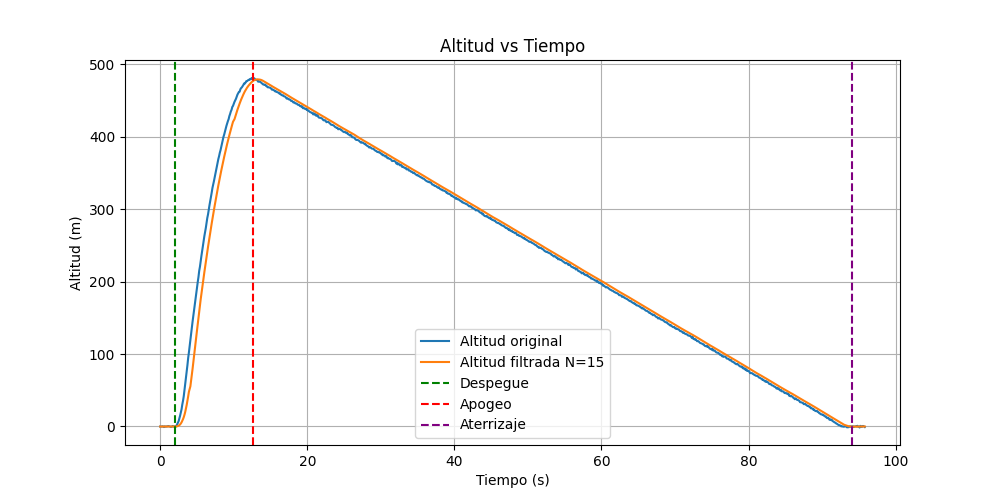
\includegraphics[width=0.82\textwidth,height=4.3cm,keepaspectratio]{altitude_plot.png}
\caption{Altitud respecto al tiempo y eventos detectados.}
\end{figure}

\begin{figure}[H]
\centering
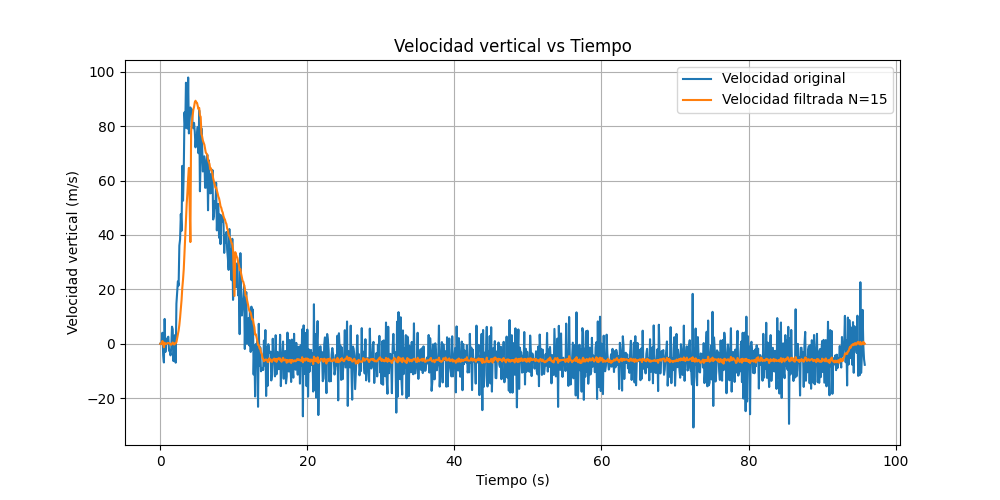
\includegraphics[width=0.82\textwidth,height=4.3cm,keepaspectratio]{velocity_plot.png}
\caption{Velocidad vertical original y filtrada.}
\end{figure}

\section{Conclusiones}

Se logró integrar la generación, depuración, filtrado y análisis de datos en un sistema funcional. La eliminación de registros corruptos permitió trabajar con datos válidos y obtener métricas del vuelo, además de representar gráficamente su comportamiento.

Sin embargo, los algoritmos de procesamiento y detección pueden perfeccionarse para responder mejor ante el ruido y las variaciones de las mediciones. Como mejoras futuras, se propone optimizar las funciones utilizadas y realizar pruebas con datos reales para evaluar el comportamiento del sistema fuera de un entorno simulado.

\newpage

\section{Bitácora de obstáculos}

Durante el desarrollo se presentaron principalmente tres dificultades:

\begin{enumerate}
\item \textbf{Falta de experiencia con Python.} Al principio tuve dificultades para comprender la estructura del código y el funcionamiento de algunas funciones. Utilicé los mensajes de error para localizar los problemas, revisar si las funciones eran adecuadas y realizar las correcciones correspondientes.

\item \textbf{Errores de sintaxis y ejecución.} En ocasiones, el desorden del código o el uso incorrecto de ciertos caracteres impedía su ejecución. Para resolverlo revisé las indicaciones del intérprete y corregí las partes señaladas hasta conseguir que el programa funcionara.

\item \textbf{Uso de plataformas y formatos.} Tuve dificultades iniciales para comprender el orden y funcionamiento de herramientas como GitHub y los formatos de trabajo. Lo resolví mediante pequeños tutoriales y revisando metódicamente cada sección para identificar patrones y comprender su uso.
\end{enumerate}

Estas dificultades me permitieron familiarizarme con herramientas que no dominaba previamente y comprender mejor el proceso de desarrollo y documentación de un proyecto técnico.

\section{Referencias y uso de IA}

Se consultaron videos de YouTube y minicursos para comprender conceptos y familiarizarse con las herramientas utilizadas.

\textbf{Uso de inteligencia artificial:} se utilizó ChatGPT como apoyo para generar y comprender código, interpretar errores de ejecución, entender el funcionamiento de las herramientas y orientar la documentación del proyecto. Las propuestas se revisaron y ajustaron durante el desarrollo.

\end{document}
